%iffalse           
\let\negmedspace\undefined
\let\negthickspace\undefined
\documentclass[journal,12pt,onecolumn]{IEEEtran}
\usepackage{cite}
\usepackage{amsmath,amssymb,amsfonts,amsthm}
\usepackage{algorithmic}
\usepackage{graphicx}
\usepackage{textcomp}
\usepackage{xcolor}
\usepackage{txfonts}
\usepackage{listings}
\usepackage{enumitem}
\usepackage{mathtools}
\usepackage{gensymb}
\usepackage{comment}
\usepackage[breaklinks=true]{hyperref}
\usepackage{tkz-euclide} 
\usepackage{listings}
\usepackage{gvv}                                        
\def\inputGnumericTable{}                                 
\usepackage[latin1]{inputenc}                                
\usepackage{color}                                            
\usepackage{array}                                            
\usepackage{longtable}                                       
\usepackage{calc}                                             
\usepackage{multirow}                                         
\usepackage{hhline}                                           
\usepackage{ifthen}                                           
\usepackage{lscape}

\newtheorem{theorem}{Theorem}[section]
\newtheorem{problem}{Problem}
\newtheorem{proposition}{Proposition}[section]
\newtheorem{lemma}{Lemma}[section]
\newtheorem{corollary}[theorem]{Corollary}
\newtheorem{example}{Example}[section]
\newtheorem{definition}[problem]{Definition}
\newcommand{\BEQA}{\begin{eqnarray}}
\newcommand{\EEQA}{\end{eqnarray}}
\newcommand{\define}{\stackrel{\triangle}{=}}
\theoremstyle{remark}
\newtheorem{rem}{Remark}
\usepackage{circuitikz}
\begin{document}

\bibliographystyle{IEEEtran}
\vspace{3cm}
\title{Assignment-2}
\author{EE224BTECH11044 - Muthyala Koushik% <-this % stops a space
}
\maketitle
\bigskip

\textbf{\section{Vector Arithmetic(CBSE)}}

\textbf{Question:} AOBC is a rectangle whose three vertices are vertices $\vec{A}\brak{0,3}, \vec{O}\brak{0,0}$ and $\vec{B}\brak{5,0}$. The length of its diagonal is \\ 

\solution  Direction vector of $\vec{AB}: m=\vec{B}-\vec{A}$
           \begin{align}
		   \vec{AB}=\myvec{5\\0}-\myvec{0\\3}=\myvec{5\\-3}
	   \end{align}	   
	   length of $\vec{AB}$(Diagonal):$\norm{\vec{m}}^2=mm^t$
	   \begin{align}
		   \norm{\vec{AB}}^2&=\myvec{5 -3}\myvec{5\\-3}\\
		      \norm{\vec{AB}}^2&=5^2+\brak{-3}^2\\
		       \norm{\vec{AB}}^2&=25+9\\
		       \norm{\vec{AB}}^2&=34\\
		   \norm{\vec{AB}}&=\sqrt{34}
	   \end{align}
	   so, length of diagonal=$\sqrt{34}$.

\begin{figure}[h!]
	\centering
	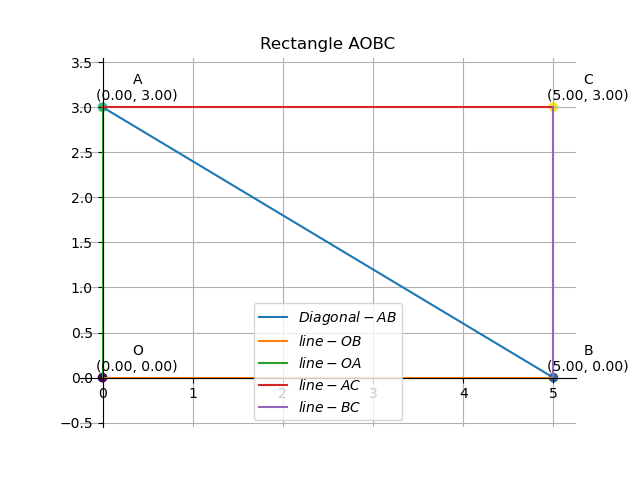
\includegraphics[width=0.6\linewidth]{figs/fig-1.png}
	\caption{The plot of the rectangle AOBC}
\end{figure}


\end{document}
